\chapter{Parsing}
\label{ch:parsing}

\section{Inleiding}
Het basisidee van parsing is om een string van tokens te analyseren en kijken of deze syntactisch geldig zijn.

\QA{Waarom gaan we context-vrije grammatica gebruiken in plaats van reguliere expressies om de tokens van een lexer te parsen?}{Reguliere expressies kan geen recursie uitdrukken. Ook kan de eis voor gebalanceerde haakjes niet uitgedrukt worden met reguliere expressies.
}

\section{Context-vrije grammatica}
\begin{itemize}
	\item Een \textbf{taal} is een verzameling \textbf{strings}.
	\item Een \textbf{string} is een eindige sequentie \textbf{symbolen} uit een \textbf{alfabet}.
	\item Analogie met een parser:
	\begin{itemize}
		\item De broncode levert de strings op via lexicale analyse.
		\item De lexicale tokens zijn de symbolen.
		\item Het alfabet is de verzameling tokentypes die gegenereerd worden door de lexicale analyzer.
	\end{itemize}
	\item De taal van een context-vrije bevat alle strings die met productieregels kan afgeleidt worden.
	\item Context-vrije grammatica definieert de \textbf{syntax} van de taal.
\end{itemize}

\subsection{Afleiden van een zin}
Grammatica \ref{fig:vb_grammatica_1} toont een voorbeeldsyntax voor lusloze programma's. Een voorbeeld van een zin is:

\begin{grammarfigure}
	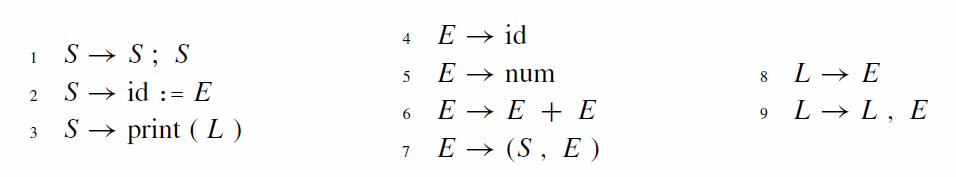
\includegraphics[width=\textwidth]{vb_grammatica_1}
	\caption{Een syntax voor een lusloos programma.}
	\label{fig:vb_grammatica_1}
\end{grammarfigure}


\begin{equation}\label{eqn:voorbeeldzin}
\texttt{id := num ; id := id + (id := num + num, id)}
\end{equation}


die bijvoorbeeld afgeleidt is door de lexer van:
$$\texttt{a := 7; b := c + (d := 5 + 6, d)}$$

Het afleiden van een zin start altijd met een \textbf{startsymbool}, die twee vormen kan aannemen:
\begin{enumerate}
	\item Het startsymbool kan enerzijds het eerste symbool zijn.
	\item Anderzijds wordt het startsymbool expliciet aangeduid zoals bijvoorbeeld $P \rightarrow S\$$, met \$ het stopsymbool.
\end{enumerate}

\begin{lstlisting}[caption={Het afleidingsproces.},label={lst:vb_afleiding},captionpos=b,escapeinside={(*}{*)}]
(*\uline{S}*)
S ; (*\uline{S}*)
(*\uline{S}*) ; id := E
id := (*\uline{E}*) ; id := E
id := num ; id := (*\uline{E}*)
id := num ; id := E + (*\uline{E}*)
id := num ; id := (*\uline{E}*) + (S, E)
id := num ; id := id + ((*\uline{S}*), E)
id := num ; id := id + (id := (*\uline{E}*), E)
id := num ; id := id + (id := E + E, (*\uline{E}*))
id := num ; id := id + (id := (*\uline{E}*) + E, id)
id := num ; id := id + (id := num + (*\uline{E}*), id)
id := num ; id := id + (id := num + num, id)
\end{lstlisting}

Code \ref{lst:vb_afleiding} toont een illustratie van hoe het afleidingsproces te werk gaat, toegepast op voorbeeldzin \ref{eqn:voorbeeldzin}. Bij elke iteratie wordt het niet-terminale token dat onderlijnt is verwerkt.

\QA{Is dit een linkse of een rechtste afleiding?}{Geen van beide, omdat zowel de meest linkse als de meeste rechtse token verwerkt kan worden.
}

Figuur \ref{fig:vb_tree_1} toont de bijhorende parse tree. Hier zijn de bladeren ook een verzameling van terminale tokens. De taak van een parser is om de bijhorende boom op te stellen, uitgaande van enkel de bladeren.

\begin{figure}
	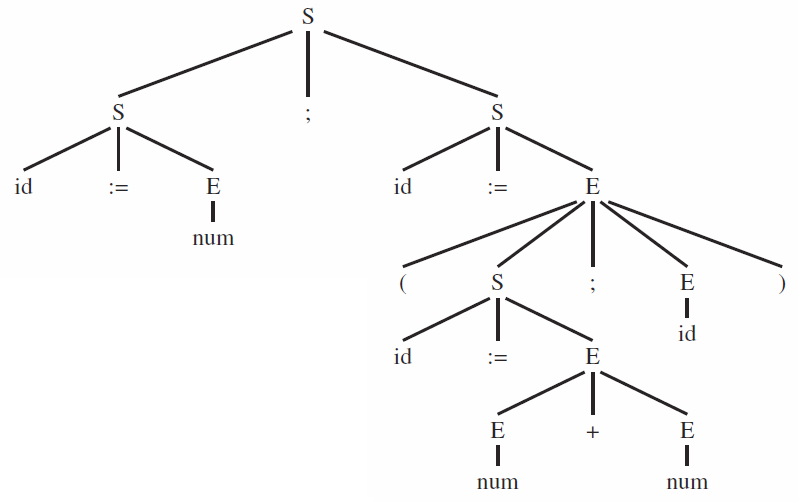
\includegraphics[width=\textwidth]{vb_tree_1}
	\caption{De bijhorende parse tree voor voorbeeldzin \ref{eqn:voorbeeldzin}.}
	\label{fig:vb_tree_1}
\end{figure}


\subsection{Ambigue grammatica}
\QA{Stel dat we Grammatica \ref{fig:vb_grammatica_1} hebben. Wat gebeurt er voor het statement (zonder rode of blauwe haakjes) \texttt{a := {\color{red}(}x + {\color{blue}(}y{\color{red})} + z{\color{blue})}}?}{Dit is een voorbeeld van een ambigue grammatica. Aan de hand van de grammatica is het onmogelijk om slechts één parse tree op te bouwen. Figuur \ref{fig:ambigious_grammar_tree} toont beide parse trees voor het statement. Bij de linkse boom worden de rode haakjes gebruikt terwijl be de rechtse boom de blauwe haakjes gebruikt worden.
}

\begin{figure}
	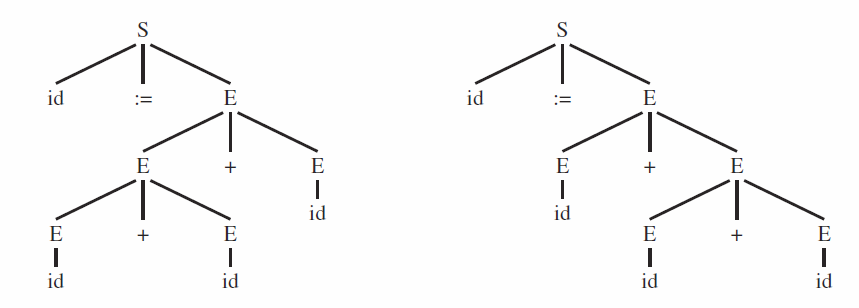
\includegraphics[width=\textwidth]{ambigious_grammar_tree}
	\caption{Voor Grammatica \ref{fig:vb_grammatica_1} kunnen er twee parse trees opgebouwd worden voor het statement \texttt{a := x + y + z}.} 
	\label{fig:ambigious_grammar_tree}
\end{figure}

Bij een plus-operatie is dit niet heel belangrijk aangezien het toch associatief is, maar bij niet-associatieve operaties is dit duidelijk niet goed.

\subsection{Grammatica disambiguëren}
Een grammatica hoeft niet perse de regels van de wiskunde te volgen. Daarom is het automatiseren ook moeilijk, omdat het afhangt van welke semantiek gewenst is. Er kan bijvoorbeeld gesteld worden dat:
\begin{itemize}
	\item * en / voorrang heeft op + en -,
	\item a + b + c = (a + b) + c, dus + is links associatief.
\end{itemize}
Om dit te realiseren worden er \textbf{expressie}, \textbf{termen} en \textbf{factoren} ingevoerd. Op die manier kan Grammatica \ref{grammar:3_5} omgevormd worden tot \ref{grammar:3_8}.

\begin{grammarfigure}
	\centering
	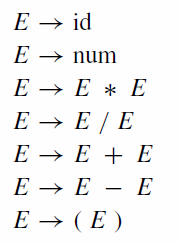
\includegraphics[width=0.25\textwidth]{grammar_3_5}
	\caption{Een ambigue grammatica. Hier wordt de regel dat * en / voorrang heeft op + en - niet gerespecteerd. }
	\label{grammar:3_5}
\end{grammarfigure}
\begin{grammarfigure}
	\centering
	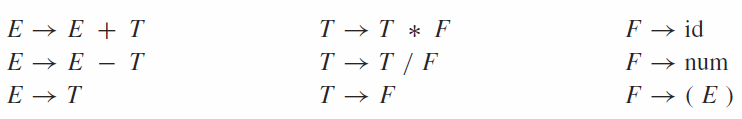
\includegraphics[width=\textwidth]{grammar_3_8}
	\caption{Grammatica \ref{grammar:3_5} kan hervormt worden, door termen $T$ en factoren $F$ in te voeren. Deze termen dwingen de volgorde van operaties en associativiteit vast.}
	\label{grammar:3_8}
\end{grammarfigure}


\section{Predictive Parsing}
Sommige grammatica's kunnen eenvoudig geparsed worden met een \textbf{recursive descent parser}. Voor elke niet-terminal is er een overeenkomstige functie. In elke functie is er een switch clause voor elke productieregel die door de niet-terminal kan gegenereerd worden. Niet-terminals worden recursief aangeroepen terwijl terminals verwerkt worden.

Code \ref{code:recursive_descent_parser} toont een voorbeld van zo een recursive descent parser toegepast op Grammatica \ref{grammar:3_11}.

\begin{grammarfigure}
	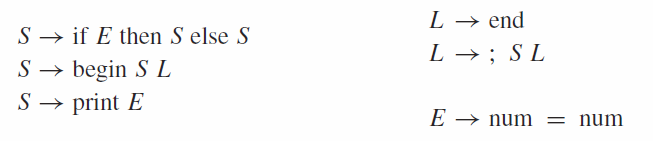
\includegraphics[width=\textwidth]{grammar_3_11}
	\caption{}
	\label{grammar:3_11}
\end{grammarfigure}

\begin{lstlisting}[caption={Een recursive descent parser gebaseerd op Grammatica \ref{grammar:3_11}},label={code:recursive_descent_parser},captionpos=b]
enum token {IF, THEN, ELSE, BEGIN, END, PRINT, SEMI, NUM, EQ};
extern enum token getToken(void);

enum token tok;
void advance() {tok = getToken();}
void eat(enum Token t) {if (tok==t) advance(); else error();}

void S(void) {switch(tok){
	case IF:    eat(IF); E(); eat(THEN); S(); eat(ELSE); S(); break;
	case BEGIN: eat(BEGIN); S(); L(); break;
	case PRINT: eat(PRINT); E(); break;
	default:    error();
}}
	
void L(void) {switch(tok){
	case END:  eat(END); break;
	case SEMI: eat(SEMI); S(); L(); break;
	default:   error();
}}

void E(void) {
	eat(NUM) ; eat(EQ) ; eat(NUM);
}
\end{lstlisting}

Een recursive descent parser werkt enkel als het eerste terminale symbool van een subexpressie genoeg informatie oplevert. Om dit te bepalen worden \texttt{FIRST} sets geïntroduceerd.

\subsection{First and follow sets}
Om de begrippen \textbf{first set} en \textbf{follow set} uit te leggen wordt Grammatica \ref{grammar:3_12} gebruikt.
\begin{grammarfigure}
	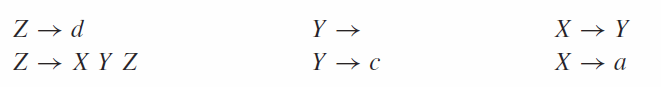
\includegraphics[width=\textwidth]{grammar_3_12}
	\caption{}
	\label{grammar:3_12}
\end{grammarfigure}
\begin{itemize}
	\item \textbf{nullable($X$)} $\rightarrow$ boolean: true als $X$ de lege string kan afleiden.
	
	We zien dat nullable($Y$) zeker waar is voor Grammatica \ref{grammar:3_12}. We kunnen echter vanuit $X$ ook naar de lege string gaan via $X \rightarrow Y \rightarrow \epsilon$, maar niet vanuit $Z$.
	
	\begin{table}[h]
		\centering
		\begin{tabular}{c | c c c}
	      & nullable & FIRST & FOLLOW \\
	      \hline
		X & yes & & \\
		Y & yes & & \\
		Z & no & & 
		\end{tabular}
	\end{table}
	
	\item \textbf{FIRST($\gamma$)}: verzameling terminals waarmee strings kunnen beginnen die van expressie $\gamma$ kunnen afgeleid worden.
	
	Uitgewerkt voor de drie symbolen:
	\begin{itemize}
		\item[$X:$] Vanuit $X$ zijn er twee mogelijkheden: $X \rightarrow a$ en $X \rightarrow Y$. We zien dat $a$ een terminal is dus die behoort al zeker tot de \texttt{FIRST} set. Vanuit $Y$ kan ook nog de lege string en $c$ bereikt worden. Hieruit volgt \texttt{FIRST}($X$) = $\{a\;c\}$.
		\item[$Y:$] Vanuit $Y$ kan enkel $c$ bereikt worden: \texttt{FIRST}($Y$) = $\{c\}$.
		\item[$Z:$] In eerste instantie kan $Z$ direct $d$ bereiken, dus die zit zeker in de \texttt{FIRST} set. Aangezien ook de productieregel $Z \rightarrow X\;Y\;Z$ bestaat en zowel $X$ als $Y$ nullable zijn, kan zowel de \texttt{FIRST} set van $X$ als van $Y$ overgenomen worden zodat \texttt{FIRST}($Z$) = $\{a\;c\;d\}$
	\end{itemize}

	\begin{table}[h]
	\centering
	\begin{tabular}{c | c c c}
			& nullable & FIRST & FOLLOW \\
			\hline
			X & yes & a c & \\
			Y & yes & c & \\
			Z & no & a c d & 
		\end{tabular}
	\end{table}
	
	\item \textbf{FOLLOW($X$)}: is de verzameling van terminals $t$ die meteen op $X$ kunnen volgen, dus waarvoor de afleiding $Xt$ bestaat. 
	Uitgewerkt voor de drie symbolen:
	\begin{itemize}
		\item[$X:$]  De regel $Z \rightarrow X Y Z$ legt vast dat $X$ door $Y$ en $Z$ kan gevolgd worden. De terminalen dat $Y$ en $Z$ kunnen genereren zijn respectievelijk $c$ en $d$ zodat die zeker al in de \texttt{FOLLOW} set zitten van $X$. Dezelfde regel $Z \rightarrow X Y Z$ kan ook $X Y X Y Z$ genereren. 
		Als $Y$ de lege string afleidt, dan kan de eerste $X$ gevolgd worden door de tweede $X$ die $a$ kan afleiden. De terminaal $a$ zit dus ook in de \texttt{FOLLOW} set van $X$ zodat \texttt{FOLLOW}($X$) = $\{a\;c\;d\}$.
		
		
		\item[$Y:$] Dezelfde redenering geldt voor $Y$: aangezien $Z$ een recursieve definitie is en het alle andere niet-terminalen bevat, is \texttt{FOLLOW}($Y$) = $\{a\;c\;d\}$. 
		\item[$Z:$] Er is geen enkele productie waarbij er een terminaal of niet-terminaal na $Z$ komt. Daarom is de \texttt{FOLLOW} set van $Z$ leeg.
	\end{itemize}
	\begin{table}[h]
		\centering
		\begin{tabular}{c | c c c}
			& nullable & FIRST & FOLLOW \\
			\hline
			X & yes & a c & a c d\\
			Y & yes & c & a c d\\
			Z & no & a c d & 
		\end{tabular}
	\end{table}
\end{itemize}

Algoritme \ref{algo:first_follow_nullable} is een fixpoint algoritme die de first, follow en nullable berekent.

\begin{lstlisting}[caption={Iteratieve berekening van FIRST, FOLLOW en nullable},label={algo:first_follow_nullable},captionpos=b,escapeinside={(*}{*)}]
(*\textbf{for}*) each terminal symbol Z
  FIRST[Z] (*$\leftarrow$*) {Z}
(*\textbf{repeat}*) 
  (*\textbf{for}*) each production (*$X \rightarrow Y_1Y_2...Y_k$*)
    (*\textbf{for}*) each (*$i$*) from 1 to (*$k$*), each (*$j$*) from (*$i + 1$*) to (*$k$*),
      (*\textbf{if}*) all the (*$Y_i$*) are nullable
        (*\textbf{then}*) nullable[X] (*$\leftarrow$*) true
      (*\textbf{if} $Y_1 \cdot\cdot\cdot Y_{i - 1}$*) are all nullable 
        (*\textbf{then}*) FIRST[X] (*$\leftarrow$*) FIRST[X] (*$\cup$*) FIRST[(*$Y_i$*)]
      (*\textbf{if} $Y_{i + 1} \cdot\cdot\cdot Y_{k}$*) are all nullable 
        (*\textbf{then}*) FOLLOW[(*$Y_i$*)] (*$\leftarrow$*) FOLLOW[(*$Y_i$*)] (*$\cup$*) FOLLOW[(*$X$*)]
      (*\textbf{if} $Y_{i + 1} \cdot\cdot\cdot Y_{j - 1}$*) are all nullable 
        (*\textbf{then}*) FOLLOW[(*$Y_i$*)] (*$\leftarrow$*) FOLLOW[(*$Y_i$*)] (*$\cup$*) FIRST[(*$Y_i$*)]
(*\textbf{until}*) FIRST, FOLLOW and nullable did not change in this iteration
\end{lstlisting}



\subsection{Opstellen Predictive Parsing Tabel}
Stel dat we een niet-terminaal $X$ hebben en een volgende input token $T$, hoe kan de beste productieregel gekozen worden? De informatie kan geëncodeerd worden in een twee-dimensionale \texttt{predictive parsing} tabel. De tabel wordt opgesteld door elke productie $X \rightarrow \gamma$ in rij $X$ en kolom $T$ te zetten voor elke $T \in \texttt{FIRST}(\gamma)$. Ook als $\gamma$ nullable is, wordt de productie in rij $X$ en kolom $T$ geplaatst voor elke $T \in \texttt{FOLLOW}[X]$. Figuur \ref{fig:predictive_parsing_table} toont de bijhorende tabel voor grammatica \ref{grammar:3_12}.
\begin{figure}
	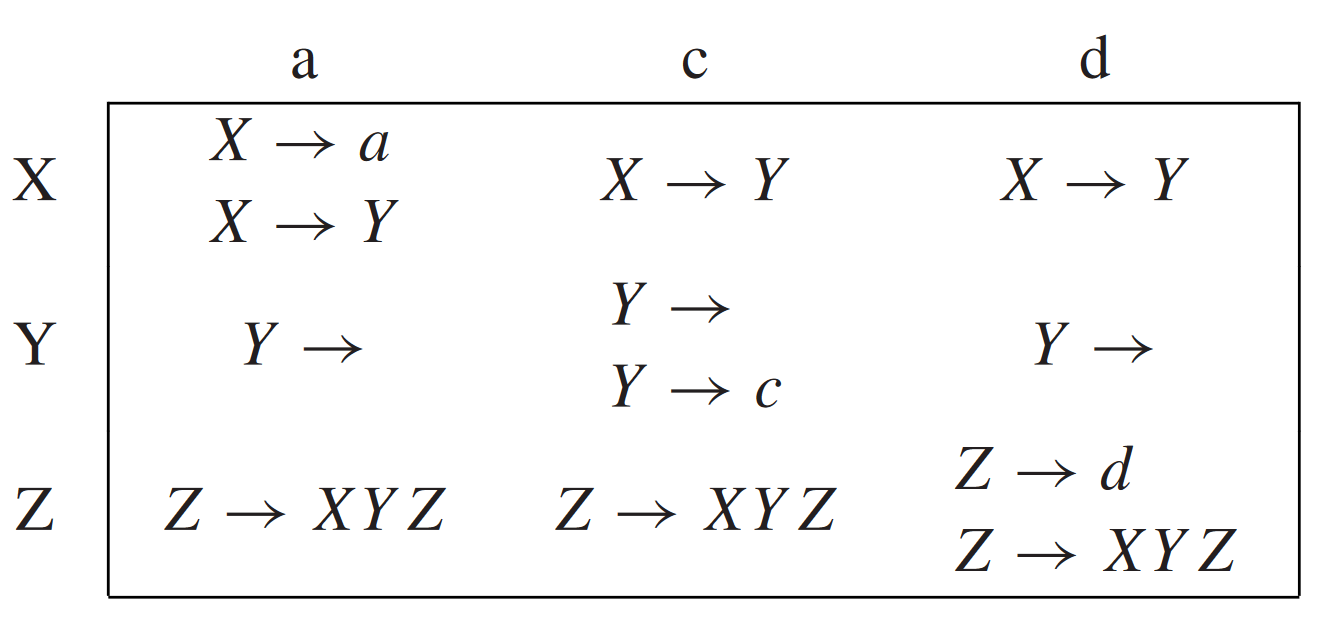
\includegraphics[width=\textwidth]{predictive_parsing_table}
	\caption{Predictive parsing tabel voor \ref{grammar:3_12}}.
	\label{fig:predictive_parsing_table}
\end{figure}

Uitbreiden definitie van first naar strings:
\begin{itemize}
	\item \texttt{FIRST($W\gamma$)} = \texttt{FIRST($W$)} als niet nullable($W$)
	\item \texttt{FIRST($W\gamma$)} = \texttt{FIRST($W$)} $\cup$ \texttt{FIRST($\gamma$)} 
\end{itemize}

Aangezien er meerdere producties zijn per cel, zal predictive parsing niet werken. Dit komt overeen met het feit dat de grammatica ambigue is.

\subsection{LL(1) Parsers}
Grammatica's waarbij de predictive parsing tabellen geen duplicate entries per cel bevat worden \texttt{LL(1)} grammatica's genoemd. Een recursive-descent parser is een voorbeeld van een \texttt{LL(1)} parser.
\begin{itemize}
	\item Elk vak in de tabel bevat slechts 1 productieregel.
	\item Left-to-right parse: begin vooraan in broncode en verwerk van links naar rechts. 
	\item Leftmost-derivation: 
	\item 1-symbol lookahead: Er wordt slechts één symbool vooraf bekeken.
	\item LL($k$):
	\begin{itemize}
		\item $k$ symbolen vooraf bekijken. De first sets bevatten sequenties van $k$ terminals.
	\end{itemize}
	
	\alert Mogelijke problemen:
	\begin{itemize}
		\item Linkse recursie.
		\begin{itemize}
			\item \textbf{Probleem}: Veronderstel volgende grammatica:
			\begin{equation*}
				\begin{split}
					E & \rightarrow E + T \\
					E & \rightarrow T
				\end{split}
			\end{equation*}
			Er zullen duplicate waarden in de predictive parsing tabel voorkomen omdat $\texttt{FIRST(T)} \in \texttt{FIRST(E + T)}$
			\item \textbf{Oorzaak}: $E$ verschijnt als eerste symbool in de rechterkant van een $E$-productie.
			\item \textbf{Oplossing}: Herschrijf de productie met rechtse recursie.
			\begin{equation*}
				\begin{split}
				E &\rightarrow T E' \\
				E'& \rightarrow + T E' \\
				E'& \rightarrow 
				\end{split}
			\end{equation*}
		\end{itemize} 
		\item Linkse factorisatie.
		\begin{itemize}
			\item \textbf{Probleem}: De parser kan geen onderscheid maken tussen twee gelijkaardige strings.
			\begin{equation*}
				\begin{split}
				S &\rightarrow \hbox{if } E \hbox{ then } S \hbox{ else } S \\
				S &\rightarrow \hbox{if } E \hbox{ then } S 
				\end{split}
			\end{equation*}
			\item \textbf{Oplossing}: Neem het gelijkaardige stuk samen en introduceer nieuwe niet-terminalen die de afwijkingen beschrijven.
			\begin{equation*}
			\begin{split}
			S &\rightarrow \hbox{if } E \hbox{ then } S X \\
			X &\rightarrow  \\
			X &\rightarrow \hbox{else } S
			\end{split}
			\end{equation*}
			
		\end{itemize}
	\end{itemize}
	\item Error recovery is mogelijk.
	\alert Beslissing nemen na $k$ symbolen blijft een zwakte.
	
\end{itemize}

\subsection{Error Recovery}
Probleem: pseudocode voor error. We willen geen compiler die geen nuttige foutboodschappen kan geven. Compiler mag ook niet stoppen bij eerste fout, omdat meerdere fouten nog verder kunnen voorkomen.
\begin{itemize}
	\item Gewoon een print statement = vrij slechte methode aangezien er geen tokens opgegeten worden. De parser doet voort alsof hij F en T' al geparsed heeft. De parser komt in foute toestand.
	\item Print statement combineren met de skipto functie, die tokens zal opeten totdat er een token tegenkomt die in de follow set zit. Alle karakters die niet in de follow zitten, zal nog deel uitmaken van de subexpressie. 
\end{itemize}

\section{LR($k$) parser}
Het probleem met $LL(k)$ parsers is dat ze moeten voorspellen welke productieregel dat ze moeten gebruiken op basis van de eerste $k$ tokens. Een $LR(k)$ parser stelt dit uit tot dat de $k$ input tokens overeenkomen met een complete productieregel.
\begin{itemize}
	\item Left-to-right parse.
	\item \underline{Rightmost}-derivation.
	\item $k$-token lookahead.
	\item Werkt met een inputstroom en een stapel.
	\item Twee mogelijke acties:
	\begin{itemize}
		\item \textbf{Shift:} verplaats een token van de inputstroom op een stapel.
		\item \textbf{Reduce:} kies een regel $X \rightarrow A B C$; Stel dat de stapel $[C, B, A]$ bevat, kunnen deze alle drie gepopt en vervangen worden door $X$.
	\end{itemize}
	\item Toestandsautomaat:
	\begin{itemize}
		\item Stapel houdt token bij en toestand.
		\item Toestand en $k$ lookahead symbolen in de input bepalen de volgende actie.
		\item Implementeren aan de hand van een toestandstransitietabel.
	\end{itemize}
\end{itemize}

\section{Local Error Recovery}